
\documentclass[a4paper]{IEEEtran}

% *** CITATION PACKAGES ***
%
\usepackage{cite}
% cite.sty was written by Donald Arseneau
% V1.6 and later of IEEEtran pre-defines the format of the cite.sty package
% \cite{} output to follow that of the IEEE. Loading the cite package will
% result in citation numbers being automatically sorted and properly
% "compressed/ranged". e.g., [1], [9], [2], [7], [5], [6] without using
% cite.sty will become [1], [2], [5]--[7], [9] using cite.sty. cite.sty's
% \cite will automatically add leading space, if needed. Use cite.sty's
% noadjust option (cite.sty V3.8 and later) if you want to turn this off
% such as if a citation ever needs to be enclosed in parenthesis.
% cite.sty is already installed on most LaTeX systems. Be sure and use
% version 5.0 (2009-03-20) and later if using hyperref.sty.
% The latest version can be obtained at:
% http://www.ctan.org/pkg/cite
% The documentation is contained in the cite.sty file itself.

\usepackage{graphicx}
\usepackage{picins}

% *** GRAPHICS RELATED PACKAGES ***
%
\ifCLASSINFOpdf
  % \usepackage[pdftex]{graphicx}
  % declare the path(s) where your graphic files are
  % \graphicspath{{../pdf/}{../jpeg/}}
  % and their extensions so you won't have to specify these with
  % every instance of \includegraphics
  % \DeclareGraphicsExtensions{.pdf,.jpeg,.png}
\else
  % or other class option (dvipsone, dvipdf, if not using dvips). graphicx
  % will default to the driver specified in the system graphics.cfg if no
  % driver is specified.
  % \usepackage[dvips]{graphicx}
  % declare the path(s) where your graphic files are
  % \graphicspath{{../eps/}}
  % and their extensions so you won't have to specify these with
  % every instance of \includegraphics
  % \DeclareGraphicsExtensions{.eps}
\fi

% *** MATH PACKAGES ***
\usepackage{amsmath}
\usepackage{scrextend}


\hyphenation{op-tical net-works semi-conduc-tor}

\usepackage{lipsum}
\makeatletter
\def\footnoterule{\relax%
  \kern-5pt
  \hbox to \columnwidth{\hfill\vrule width 0.5\columnwidth height 0.4pt\hfill}
  \kern4.6pt}
\makeatother

\begin{document}

\title{From textual to structured Web API Descriptions\\ \large Knowledge Discovery and Data Mining Seminar 2017 }


\author{Selcuk~Aklanoglul,
        Han~Che,
        Caroline~Dieterich,
        Marcel~Ruoff,
        Jan-Peterl~Schmidt  \\
Karlsruhe Institute of Technology \\
Sebastian~Baader \\
Department Applied Informatics and  Formal Description Methods (AIFB)  \\
Karlsruhe Institute of Technology

}



\maketitle

\begin{abstract}
In this study, we investigate the possibility of using Knowledge Discovery and Data Mining approaches to transform human written textual Web Application Programming Interface
(API) descriptions into structural descriptions, which
can be consumed by machines. The central vision
is to provide a solution, which ultimately allows
machines to interchange APIs with similar purposes
automatically. A use case would be to replace non-
responding data providing API (e.g. weather,
location, news) with another. Using descriptions
provided by ProgrammableWeb, with over 15000
APIs one of the most prominent public API library,
we conducted multiple steps of data cleaning and
preprocessing followed by machine learning
algorithms (K-Means, DBSCAN) to create clusters,
which we validated manually. With an average only
68,3 Words per descriptions (45,6 after
preprocessing) our results suggests, that the
needed quantity for text mining and clustering was insufficiently met. Our clusters were thus also
inconclusive.
\end{abstract}


\IEEEpeerreviewmaketitle

\section{Introduction}
\IEEEPARstart{A}{pplication} Programming Interfaces (API) are not just a way to give developers access to software or services anymore. A whole business economy has established around the concept of exposing APIs in order to provide access and services. Programmable Web currently lists 15839 public available API (State June 2017). While ProgrammableWeb represent as set of manually collected APIs, APIHound claims to have crawled and indexed over 50000 APIs.
According to 3scale CEO Steve Willmott, eBay, Flickr, and Salesforce were among the companies that helped popularize the API [1] leading towards entire business models evolving around API services and strategies. Along came new terminologies to define this industry such as API Economy and Business to Developer (B2D).

API Economy is defined as the positive affect APIs can have on an organization’s profitability. [2]
It can be loosely compared to the prestige of patents plaques. The more holistic a company provides APIs the more developers can make use of it. Well documented API’s attracts developers to either actively consume APIs or even build their own business on top of it.

\begin{figure}[!t]
\centering
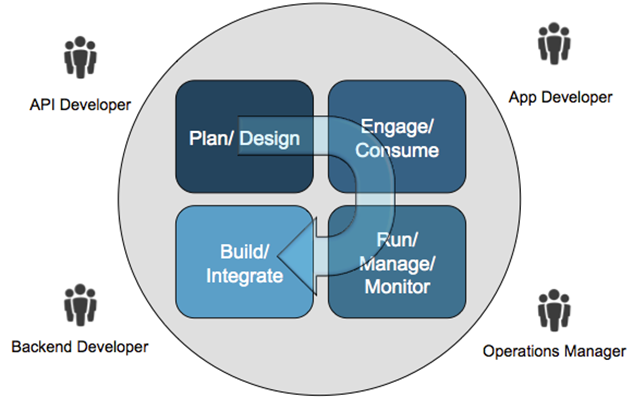
\includegraphics[width= 3in]{img/APIcycle.png}
\caption{MuleSoft on API Econom}
\label{fig_sim}
\end{figure}

Business to Developer (B2D), implies a business model, which is targeting developers as customers. With the movement of open source and cloud technologies developers rarely have to rely on in-house resources anymore. Instead of building a new project form the ground up, developers can access numerous available 3rd party libraries to reduce developing time and effort. For certain services and libraries, they are event willing to pay a premium.

With the rise of API demand and supply, the API Economy calls for a product market similar ecosystem. While human customers have various sources to evaluate a product or service (or API), currently no solutions exist which lets machines choose their own source of information or functionality. Most APIs are hardcoded into the application or software. The current digital market boasts of interconnectedness. Every product is in one way or the other connected to the internet and thus “made smart”, yet any or especially so called breaking changes to the API will require developers to update their code manually. 
For our research paper, we investigate one the basic requirements for machines to accomplish such breaking changes on their own. Our focus is on whether we can transform textual description to machine-usable structural descriptions, by using ProgrammableWeb, one of the largest API aggregation open source available.

\section{Datasets and Crawling}
%rechtsbündige grafik
%\piccaption{Amount of working links in Programmable Web} 
%\parpic[r]{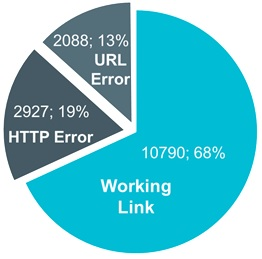
\includegraphics[width=1.5in]{img/pie.png}} 
Prior to our research and development, we looked for suitable datasets with good quality. There was not much research done in this field, therefore we had to look for different alternatives, which will be described in the following Sections. Section II.A describes the Linked Web API dataset and the issues. Section II.B deals with the dataset crawled from Programmable Web  \footnote[1]{https://www.programmableweb.com} and Section II.C shows an alternative way to get data from Google.
\begin{figure}[!t]
\centering
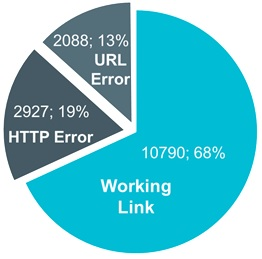
\includegraphics[width= 2in]{img/pie.png}
\caption{Amount of working links in Programmable Web}
\label{fig_sim}
\end{figure}

\subsection{Linked Web API Dataset}
Starting point was the Linked Web API dataset [1] with 9.850 APIs. Besides short descriptions of the API, it inherits also semantic annotations and links between different attributes like title, tags and links to websites. For our purpose only the descriptions were relevant. The first inspection shows, that the descriptions were too short. Since we want to cluster the APIs on similarity based on their descriptions, those were crucial. First solution was to crawl the website of the API. This seemed to be easily done, since the dataset also had a link to the API documentation website. When checking the links, we found out that 78 \% (Fig. 1) of the links were missing. The remaining 1.500 links where leading to any subpages, but not to the actual API documentation. Therefore, crawling those sites would result in a poor data quality, since we have no control over which textual content would be crawled.

\subsection{Programmable Web Dataset}
Another approach to get usable data was, to crawl Programmable Web with over 15.800 APIs. Therefore, we constructed a crawler with the Scrapy Framework \footnote[2]{https://scrapy.org} to crawl all the data. The API descriptions from Programmable Web have an averege length of 70 words, which we assumed to be not enough. We examined the linkts to the API documentation sites, to see if we can crawl them, too. From the 15.800 APIs, about 32 \% (Fig. 2) were not working. When we investigated the links further, we found out, that approximately 30 to 45 \% of the links redirect to a subpages like  main, authentication or payment pages. This was the same issue like with the Linked Web API dataset.

\subsection{Google Crawled Dataset}
Since the links from the datasets in Section II.A and II.B were not usefull, we decided to crawl a complete new dataset from Google. We constructed a search query out of the API names with additional filters, shown in (1).
site:paypal.com “api documentation" OR “api reference” “paypal payments api”	(1)
We saved the first five results with every result being in its own key-value pair, so that we can distinguish between the ranks of the results. Our assumption was, that Google will return the best result (link to the actual API documentation website) on rank 1. We investigated a couple of those links and came to conclusion, that our assumption was false. Therefore we could not use the dataset from Google.
We decided to use the Programmable Web dataset with the limited amount of API descriptions.

\section{Preprocessing}
The preprocessing was done in three steps. First the data was cleaned, afterwards the words of API descriptions were transformed into a matrix and finally the dimensions of the matrix were reduced.

\subsection{Data Cleaning}
The data cleaning included punctuation removal, number removal, transformation to lower case, stop word removal and lemmetization. The cleaning was done with Python, for lemmatization the lemmatizer from the Natural Language Toolkit (nltk) library was used \cite{bird2009natural}. The cleaned API descriptions were saved in JSON format.

\subsection{Vectorization}
After the data cleaning, we are left with API descriptions, referenced as documents, which consist of a varying number of words, referenced as terms. Before clustering algorithms can be applied on the data it has to be transformed. The aim is to generate a matrix where every row represents an document and each column a term. The values of that matrix determine if a term is part of a description and which importance the term has. To archive this, we used the term frequency times inverse document frequency (TF-IDF) Vectorizer from the Python library scikitLearn \cite{scikit-learn}. The Vectorizer counts the frequency of a word in an API description and the frequency of that word in the whole data set. The importance of a Word then is calculated by the following formula.

\begin{equation*}
tfidf (d,t) = tf(t) * idf(d,t) 
\end{equation*}

tf(t) is the term frequency of a term in an API description. This term frequency is multiplied with the inverse document frequency which is calculated according to the following formula.

\begin{equation*}
idf (d,t) = log\left( \frac{1+n}{1+df(d,t)} \right)
\end{equation*}

N is the total number of API descriptions and df(d,t) the document frequency, the number of documents in which a term t appears. 
With the TF-IDF Vectorizer terms with a high term frequency but a low document frequency have the highest tf-idf-value and can be considered more important than terms with a lower tf-idf-value. The result of the vectorization is a spars matrix with xx dimensions.

\subsection{Latent Semantic Analysis}
A dimension reduction was not only necessary because of the size of the Matrix, but is also suggested by Ding and He 2004 \cite{ding2004k}. They showed, that a dimension reduction with the Principal Component Analysis (PCA) before the use of K-Means leads to better clustering  results. Having a huge sparse matrix makes it difficult to perform a PCA. Therefore, we used the transformer TruncatedSVD from the scikitLearn library to perform a dimension reduction \cite{scikit-learn}. The transformer uses a truncated Singular Value Decomposition (SVD) which is specially tailored to TF-IDF matrixes and therefore called Latent Semantic Analysis. This makes a centering of the data not necessary and is for that reason suitable for large sparse data sets \cite{albright2004taming}.

\section{Manual Clustering}
To be able to assess the quality of our trained clusters, we decided to manually create clusters and only evaluate (in Section V) on those manually clustered APIs. With that, we could test different clustering parameters described in Section IV and choose the best parameters. We split the dataset according to the existing categories and took the five tags: “Messaging”, “Payments”, “eCommerce”, “Mapping” and “Finance”, since they contained most of the APIs. Based on the descriptions we clustered those APIs manually, so that we receive about 30 APIs per cluster. After 2-3 days of processing, we had 26 manually created clusters with 962 APIs.

\section{Clustering}
To suggest for a given API from a user similar APIs we tried two different approaches. In our first approach we used clustering algorithms which are mostly used for data mining and knowledge discovery, data compression and pattern recognition. Mostly the field of clustering algorithms for pattern recognition were capable to solve our given problem. In our case the algorithms assigned APIs to the same cluster if they had similar wording patterns and descriptions. 
Our other approach was to create a correlation matrix which declares for each API how similar it is to a given API. To achieve this the algorithm had to calculate the distance between each API and create a square matrix for the given data.
To implement and test these approaches we used the following algorithms.

\subsection{API Clustering}
For the correlation matrix we tried to implement the algorithm introduced by Jian Wu, Liang Chen, Zibin Zheng, Michael R. Lyu and Zhaohui Wu in their Paper “Clustering Web services to facilitate service discovery”. The algorithm determines the similarity of each APIs word-vector with all the other word vectors by comparing the word in the word-vector with the normalized google distance. As a result, the algorithm produces a correlation-matrix where for any given API the distance to each other API can be withdrawn.

\begin{equation*}
Algorthm
\end{equation*}

The main advantage is that the authors already tried to solve our use-case with their algorithm and demonstrated that it could work. They also used the same pre-processing techniques to determine the word-vectors. This means we had the same initial situation.
To determine the normalized google distance, which is crucial for the determination of our results, we had to crawl google for each word combination in our word-vectors. Because we lacked the time we tried to use google ngram. Google ngram is a database with scanned books. It also provides command lines to build correlation-matrixes for given words, which would make it possible to implement the normalized google distance. Unfortunately, the current version is from 2012 which resulted in an insuperable problem. Words like “instagram” which were used in our word vectors and were crucial for interpretable results weren’t included in google ngrams. Because of this we didn’t used the implementation of this paper in our further project.

\subsection{Density-Based Clustering}
The first clustering algorithm we tried out was the density-based spatial clustering of applications with noise (DBSCAN). DBSCAN is a density based clustering algorithm grouping together closely packed data-points with a given number of neighbours required for a point to be dense ( minPts ) and a maximum distance between two neighbours in a cluster ( ε ). 

\begin{equation*}
Algorthm
\end{equation*}

The main advantage of DBSCAN is that APIs without any similar APIs in a given distance, also called noise, will be ignored an assigned to a separate cluster. This results in an undistorted result and as an information for a user that there is no similar API. 
Another advantage is that there is no fixed number of clusters because this will be optimized during the execution of the algorithm.
The decisive disadvantage is that only the distance between two neighbours in a cluster are considered in the algorithm. Resulting in an unknown width of the clusters. This means that two completely different APIs could end up in the same cluster because there is a linking chain of APIs between them. With this problem there was no assurance that the algorithm produces a logical result for our use-case.
Another problem occurred during the execution of our implementation. Given a set of 3000 APIs, number of neighbours required for a API to be consider dense of minPts = 2 and a ε = 1,2 our algorithm considered half of these APIs noise and the other half was put into clusters with an average number of seven APIs. The input can be interpreted that there only must be one other API in a distance of 1,2 around a given API. This means our input had to be very vague for any results. Because of this and the wrong assignment of APIs to the noise category we didn’t use DBSCAN for further implementation.


\subsection{K-Means Clustering}
The clustering algorithm we used for our final implementation is k-means, one of the most widely used clustering algorithm. For a given set of data-points in a n-dimensional space Rn and an integer k the algorithm determines k points, called centres, minimizing the sum of the mean square distance from the data points to their nearest centre. We are using the k-means adaptation of the Lloyed-algorithm described in Algorithm 3.

\begin{equation*}
Algorthm
\end{equation*}

The main advantage is the simplicity of the algorithm and performance. Another advantage is that because of the minimization of the mean square distance of the APIs to their centres we also minimize the distance between two APIs in the same cluster.
The main challenge of the k-means algorithm is that the integer k is fixed and can’t be optimized with the algorithm itself. To counteract this problem we split the possible number of clusters into intervals. For each interval we executed the k-means algorithm for the boarder points of the interval and compared the result of these outputs in our evaluation.
A problem that we couldn’t overcome was the inclusion of noise in our results. APIs without any similar APIs were still included in a cluster and this could distort our results.
Since we used k-means for our final implementation the results of this algorithm will be evaluated in the Evaluation.


\section{Evaluation}
K-Means in combination with LSA leaves us with three parameters that have to be determined, the cluster size, the distance metric, and the number of dimensions the input data was reduced to. To determine the best values for those parameters we run the clustering with different parameter combinations. The clusters resulting from the different combinations were then compared to the manually formed clusters. We used two different methods to determine the quality of the machine created clusters, the Jaccard coefficient together with the Rand Statistic and Precision and Recall. As a last step we selected one of the best parameter combinations to manually evaluate the correctness of the clustering. The following paragraph introduces the two different quality measurements and the process of the manual evaluation.

\subsection{Jaccard Coefficient}
As [Halkidi, 2002] \cite{halkidi2002cluster}  suggests we used Jaccard-Coefficient for quality measurement. Jaccard measures the intersection of two quantities. In our case on quantity is the manual created cluster, lets name it C, the other one is the cluster set that k-means provides, lets name it K. In formal:

\begin{equation*}
manual~Cluster~C := \{ c_1,c_2,...,c_n \}
\end{equation*}
\begin{equation*}
k-means~Cluster~K := \{ k_1,k_2,...,k_n \}
\end{equation*}

We used the approach for calculating Jaccard as described in [Halkidi, 2002]. Therefore, we build every possible pair Y in C.

\begin{equation*}
Y= ( y_1,y_2) : y_1, y_2 \in C
\end{equation*}

Furthermore, we search for Y in K. 
\begin{equation*}
\Rightarrow ~try~to~find:
\end{equation*}
\begin{equation*}
X= ( x_1,x_2) : x_1= y_1,x_2= y_2 \in K
\end{equation*}

Now we can derive for every possible X and Y whether $y_1$  and $y_2$ are in the same cluster and if $x_1$  and $x_2$ are in the same cluster. We can get the following combinations: \\
\begin{labeling}{Different-Diffr. (DD)}
\item [Same-same (SS)]  $i.e.~y_1,y_2 \in c_l; x_1,x_2∈k_h$ \\
\item [Same-Different (SD)]  $i.e.~ y_1,y_2 \in c_l; x_1 \in k_h; x_2 \notin k_h$ \\
\item [Different-Same (DS)]  $i.e.~ y_1 \in c_l; y_2 \notin c_l; x_1,x_2 \in k_h$ \\
\item [Different-Diffr. (DD)]  $i.e.~y_1 \in c_l; y_2 \notin c_l; x_1 \in k_h;x_2 \notin k_h$
\end{labeling}

We count how many SS, SD, DS and DD pairs exists. With these numbers, we can calculate the Jaccard Coefficient. We also provide Rand statistics because we can easily calculate it from the same numbers.

\begin{equation*}
Jaccard~Coefficient:~ j:= \frac{|SS|}{|SS|+|DS|+|SD|}
\end{equation*}
\begin{equation*}
Rand~statistics:~ rs:= \frac{|SS|+|DD|}{|SS|+|DS|+|SD|+|DD|}
\end{equation*}
A bigger Jaccard coefficient indicates a higher number of APIs which are in the right cluster with each other and is therefore better.

But this approach quickly showed some problems. Due to a high number of APIs in our dataset we have a huge number of operations for calculating Jaccard Coefficient. It showed that evaluation took much more time than creating the clusters with k-means. The following paragraph shows what the problem was and how we solute it.
Because of the pair-pair comparison we had to run very often through our api list. According to [Halkidi, 2002] we have to build M pairs over our api list.

\begin{equation*}
M= \frac{N*(N-1)}{2}\approx \frac{10,000*9,999}{2}=49,995,000
\end{equation*}

These nearly 50 million pairs have to be checked against the pairs build from our manual clustering list which contained nearly 1000 APIs. That means that are also nearly a half million pairs. Finally, we have to do a bit less than $50*10^6*0,5*10^6=25*10^{12}$ comparisons. This took much more time than building our clusters with k-means and was not useable due to lack of time for our work.
We tried to fix that problem with two different ideas. One is described in the next section and is about using other parameter that are not calculated by comparing pairs which decreased complexity. The other idea is easier and also fixed our problem. We were able to decrease the bigger pairs list dramatically by only building pairs that are also in our manual clustered list. Because if they are not clustered manually they cannot be used for evaluation and thus, are not necessary to be build. This is achieved by a reduction of the api list at start time of the comparison algorithm. This decreased runtime from hours to a few minutes which is quite acceptable.

\subsection{Precision and Recall}
The other idea of fixing the runtime problem was using precision and recall as coefficient for similarity. These two are also often used for cluster similarity measurement. Basically, the use the same concept with classifying if one api is true positive, false positive, true negative or false negative sorted into a clustered according to a certain set of clusters that is assumed to be correct. The advantage is that we do not need to build pairs for calculation and can decrease runtime by that.

Let assume we have to sets of APIs:
\begin{equation*}
manual~Cluster~C := \{ c_1,c_2,...,c_n \}
\end{equation*}
\begin{equation*}
k-means~Cluster~K := \{ k_1,k_2,...,k_n \}
\end{equation*}

The algorithm initially breaks down the list of apis to the amount of manually clustered api list to increase performance. 
Afterwards it takes one API from the manual clustered list and identifies its cluster. If that cluster was not evaluated already, we are looking for all other APIs that are contained in this cluster in the manual clustered list. Having a selected cluster $(c_i)$ with all its apis we are looking for the most similar cluster in the machine cluster set. Therefore, we are iterating through K and define a new list of clusters named T. If we find and api that is in $c_i$ we store the cluster id from the machine clustered list in T and count how many apis that are contained in $c_i$ are there in. If we have done this for all apis is in K we can derive from T which cluster in K is most similar to $c_i$ (the selected cluster from C, our manual clustered list). This most similar cluster is called $t_i$. From that we can easily calculate recall and precision between these two clusters by checking the four following possibilities.

\begin{labeling}{False negative (fn)}
\centering \item  [True positive (tp)] $x_n \in c_i,x_n \in t_i$
\item [False positive (fp)] $x_n \notin c_i,x_n \in t_i$
\item [True negative (tn)] $x_n \notin c_i,x_n \notin t_i$
\item [False negative (fn)] $x_n \in c_i,x_n \notin t_i$
\end{labeling}

We are counting how these four case occurred and can calculate from that precision and recall. 

\begin{equation*}
Precision= \frac{|tp|}{|tp|+|fp|}
\end{equation*}
\begin{equation*}
Recall= \frac{|tp|}{|tp|+|fn|}
\end{equation*}

With that we are able to calculate precision and recall for cluster $t_i$. Do determine the quality of K we are calculate precision and recall for each cluster and print the average for each at the end of calculation. The clustering with the overall highest precision and an overall highest recall can be considered the best clustering. For an easier comparison the F-measure is calculated. 

\begin{equation*}
F=2* \frac{Precision*Recall}{Precision+Recall}
\end{equation*}

The F-measure is the harmonic mean between Precision and Recall. The higher the value the better the quality of the clusters.

\subsection{Manual Evaluation}
We created a simple website which has two purposes. It enables an easy manual evaluation and access to anyone to use our results. The data the site is based on is a JSON file. It contains the result of the K-Means clustering with a parameter combination that had one of the best quality measures.

The user can enter a name of an API to find similar APIs. The site provides the data of our machine clustered data. It looks up similar APIs from the JSON file and provides them with a small description. The user has then the possibility to give a positive vote if a suggested API matches the one he put in or give a negative vote if not.
With the user input an overall quality measure can be calculated as the percentage of correctly clustered APIs:

\begin{equation*}
Quality= \frac{positive~votes}{all~votes}
\end{equation*}

\section{Results}
We run the evaluation with all possible combinations of the predefined values for the parameters. For the number of clusters k, 13 values between $k=1$ to $k=7500$ where chosen. With a k of one, all APIs are in one cluster and with a k of 7500 the average size of a cluster is XX. We used two different metrics for distance measurements, the Euclidian distance and the Cosine distance and did a dimension reduction dim to $dim⁡= 10$, $dim⁡= 100$, $dim⁡=  250$ and  $dim⁡= 500$ dimensions. This leaves us with $13*2*4=104$ clustering cycles. For every cycle the quality measures were calculated.

The comparison of the quality measures revealed, that they suggest different optimal k, regardless of the dim and the distance metric. The Jaccard as well as the Rand statistic have their maximum between $k=20$ and $k=50$ for all dim and distance metric combinations. Whereas the F-measure indicates an optimal number of clusters between $k=300$ and $k=700$.
The low k suggested by the Jaccard coefficient would mean that we have an average cluster size of around XX, which is too high. The optimal k of the Jaccard coefficient is also very close to the number of manually clustered APIs. It is to investigate to what extend the Jaccard coefficient is influenced by the manual clustering. To avoid any bias which might be caused in this case we put the focus of the evaluation on the precision and recall measure and therefore on the F-measure.


\begin{figure}[!t]
\centering
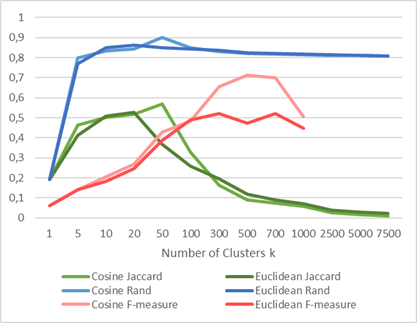
\includegraphics[width= 3.5in]{img/Jaccard.png}
\caption{Difference between Jaccard coefficient and F-messure}
\label{fig_sim}
\end{figure}

The F-measure shows a similar hight for a dimenson reduction to $dim⁡= 100$, $dim⁡= 250$ or $dim⁡= 500$ dimensions. The F-measure of a clustering with a $dim=10$ is overall lower than one of a clustering with $dim⁡= 100$, $dim⁡= 250$ or $dim⁡= 500$. 
It is not possible to make a general assumption which distance metric produces better cluster quality. It changes depending on the parameter combination. The Euclidian metric gives a gives a higher F-measure with a $dim⁡= 100$ and the cosine metric with $dim⁡= 250$ or $dim⁡= 500$.

Of all the parameter combination we tested, the parameter combinations $k⁡= 500$, $dim⁡= 500$, cosine and $k⁡= 700$, $dim⁡= 100$, euclidian had the best F-measures with 0,71 and 0,74.
The results of the K-Means clustering with the parameters $k⁡= 500$, $dim⁡= 500$, cosine were den integrated into the website. 303 APIs were evaluated through the website. The resulting quality is 59 \%.



\section{Future Work}
The classification anhand der texte und das Vorgehen funktioniert im Moment sind die ergebnisse aber noch nicht besser als Programmable Web Clustering. Was noch verbessert werden kann: 
Manuelles Clustering Verbessern
Längere Beschreibungstexte
Mehr werte für Parameter einsetzten
Mehr APIs manuell evaluieren
Parameter learning… 


\newpage





\bibliographystyle{IEEEtran}
\bibliography{quellen}




\end{document}


